% Template for PLoS
% Version 3.3 June 2016
%
% % % % % % % % % % % % % % % % % % % % % %
%
% -- IMPORTANT NOTE
%
% This template contains comments intended 
% to minimize problems and delays during our production 
% process. Please follow the template instructions
% whenever possible.
%
% % % % % % % % % % % % % % % % % % % % % % % 
%
% Once your paper is accepted for publication, 
% PLEASE REMOVE ALL TRACKED CHANGES in this file 
% and leave only the final text of your manuscript. 
% PLOS recommends the use of latexdiff to track changes during review, as this will help to maintain a clean tex file.
% Visit https://www.ctan.org/pkg/latexdiff?lang=en for info or contact us at latex@plos.org.
%
%
% There are no restrictions on package use within the LaTeX files except that 
% no packages listed in the template may be deleted.
%
% Please do not include colors or graphics in the text.
%
% The manuscript LaTeX source should be contained within a single file (do not use \input, \externaldocument, or similar commands).
%
% % % % % % % % % % % % % % % % % % % % % % %
%
% -- FIGURES AND TABLES
%
% Please include tables/figure captions directly after the paragraph where they are first cited in the text.
%
% DO NOT INCLUDE GRAPHICS IN YOUR MANUSCRIPT
% - Figures should be uploaded separately from your manuscript file. 
% - Figures generated using LaTeX should be extracted and removed from the PDF before submission. 
% - Figures containing multiple panels/subfigures must be combined into one image file before submission.
% For figure citations, please use "Fig" instead of "Figure".
% See http://journals.plos.org/plosone/s/figures for PLOS figure guidelines.
%
% Tables should be cell-based and may not contain:
% - spacing/line breaks within cells to alter layout or alignment
% - do not nest tabular environments (no tabular environments within tabular environments)
% - no graphics or colored text (cell background color/shading OK)
% See http://journals.plos.org/plosone/s/tables for table guidelines.
%
% For tables that exceed the width of the text column, use the adjustwidth environment as illustrated in the example table in text below.
%
% % % % % % % % % % % % % % % % % % % % % % % %
%
% -- EQUATIONS, MATH SYMBOLS, SUBSCRIPTS, AND SUPERSCRIPTS
%
% IMPORTANT
% Below are a few tips to help format your equations and other special characters according to our specifications. For more tips to help reduce the possibility of formatting errors during conversion, please see our LaTeX guidelines at http://journals.plos.org/plosone/s/latex
%
% For inline equations, please be sure to include all portions of an equation in the math environment.  For example, x$^2$ is incorrect; this should be formatted as $x^2$ (or $\mathrm{x}^2$ if the romanized font is desired).
%
% Do not include text that is not math in the math environment. For example, CO2 should be written as CO\textsubscript{2} instead of CO$_2$.
%
% Please add line breaks to long display equations when possible in order to fit size of the column. 
%
% For inline equations, please do not include punctuation (commas, etc) within the math environment unless this is part of the equation.
%
% When adding superscript or subscripts outside of brackets/braces, please group using {}.  For example, change "[U(D,E,\gamma)]^2" to "{[U(D,E,\gamma)]}^2". 
%
% Do not use \cal for caligraphic font.  Instead, use \mathcal{}
%
% % % % % % % % % % % % % % % % % % % % % % % % 
%
% Please contact latex@plos.org with any questions.
%
% % % % % % % % % % % % % % % % % % % % % % % %

\documentclass[10pt,a4paper]{article}  %\documentclass[10pt,letterpaper]{article}
\usepackage[top=0.85in,left=2.75in,footskip=0.75in]{geometry}

% amsmath and amssymb packages, useful for mathematical formulas and symbols
\usepackage{amsmath,amssymb}

% Use adjustwidth environment to exceed column width (see example table in text)
\usepackage{changepage}

% Use Unicode characters when possible
\usepackage[utf8x]{inputenc}

% textcomp package and marvosym package for additional characters
\usepackage{textcomp,marvosym}

% cite package, to clean up citations in the main text. Do not remove.
\usepackage{cite}

% Use nameref to cite supporting information files (see Supporting Information section for more info)
\usepackage{nameref,hyperref}

% line numbers
\usepackage[right]{lineno}

% ligatures disabled
\usepackage{microtype}
\DisableLigatures[f]{encoding = *, family = * }

% color can be used to apply background shading to table cells only
\usepackage[table]{xcolor}

% array package and thick rules for tables
\usepackage{array}

% create "+" rule type for thick vertical lines
\newcolumntype{+}{!{\vrule width 2pt}}

\usepackage{footmisc}

% create \thickcline for thick horizontal lines of variable length
\newlength\savedwidth
\newcommand\thickcline[1]{%
  \noalign{\global\savedwidth\arrayrulewidth\global\arrayrulewidth 2pt}%
  \cline{#1}%
  \noalign{\vskip\arrayrulewidth}%
  \noalign{\global\arrayrulewidth\savedwidth}%
}

% \thickhline command for thick horizontal lines that span the table
\newcommand\thickhline{\noalign{\global\savedwidth\arrayrulewidth\global\arrayrulewidth 2pt}%
\hline
\noalign{\global\arrayrulewidth\savedwidth}}


% Remove comment for double spacing
%\usepackage{setspace} 
%\doublespacing

% Text layout
\raggedright
\setlength{\parindent}{0.5cm}
\textwidth 5.25in 
\textheight 8.75in

% Bold the 'Figure #' in the caption and separate it from the title/caption with a period
% Captions will be left justified
\usepackage[aboveskip=1pt,labelfont=bf,labelsep=period,justification=raggedright,singlelinecheck=off]{caption}
\renewcommand{\figurename}{Fig}

% Use the PLoS provided BiBTeX style
\bibliographystyle{plos2015}

% Remove brackets from numbering in List of References
\makeatletter
\renewcommand{\@biblabel}[1]{\quad#1.}
\makeatother

% Leave date blank
\date{}

% Header and Footer with logo
\usepackage{lastpage,fancyhdr,graphicx}
\usepackage{epstopdf}
\pagestyle{myheadings}
\pagestyle{fancy}
\fancyhf{}
\setlength{\headheight}{27.023pt}
\lhead{
\includegraphics[width=2.0in]{PLOS-submission.eps}}
\rfoot{\thepage/\pageref{LastPage}}
\renewcommand{\footrule}{\hrule height 2pt \vspace{2mm}}
\fancyheadoffset[L]{2.25in}
\fancyfootoffset[L]{2.25in}
\lfoot{\sf PLOS}

%% Include all macros below

\newcommand{\cursedforest}{{\sc CursedForest}}
\newcommand{\lorem}{{\bf LOREM}}
\newcommand{\ipsum}{{\bf IPSUM}}

%% END MACROS SECTION

\usepackage{multirow}


%%local edits (rob)
\let\oldmarginpar\marginpar
\renewcommand\marginpar[1]{\-\oldmarginpar[\raggedleft\footnotesize #1]%hv
{\raggedright\footnotesize #1}}
\reversemarginpar
\setlength{\marginparwidth}{5cm}


\begin{document}
\vspace*{0.2in}

% Title must be 250 characters or less.
% Please capitalize all terms in the title except conjunctions, prepositions, and articles.
\begin{flushleft}
{\Large
\textbf\newline{Cursed Forest - A random forest implementation for ``big'' and ``wide'' data} % Please use "title case" (capitalize all terms in the title except conjunctions, prepositions, and articles).
}
\newline
% Insert author names, affiliations and corresponding author email (do not include titles, positions, or degrees).
\\
Aidan O'Brien\textsuperscript{1},
Piotr Szul\textsuperscript{2},
Stephanie Li\textsuperscript{3},
James Doecke\textsuperscript{3},
Nick Ellis\textsuperscript{4},
Robert Dunne\textsuperscript{5}, and
Denis C. Bauer\textsuperscript{1,*}
%, with the Lorem Ipsum Consortium\textsuperscript{\textpilcrow}
\\
\bigskip
\bf{1} Health \& Biosecurity, CSIRO, Sydney, NSW, Australia
\\
\bf{2} Data61, CSIRO, Brisbane, QLD, Australia
\\
\bf{3} Health \& Biosecurity, CSIRO, Brisbane, QLD, Australia
\\
\bf{4} Oceans \& Atmosphere, CSIRO, Brisbane, QLD, Australia
\\
\bf{5} Data61, CSIRO, Sydney, NSW, Australia
\\
\bigskip

% Insert additional author notes using the symbols described below. Insert symbol callouts after author names as necessary.
% 
% Remove or comment out the author notes below if they aren't used.
%
% Primary Equal Contribution Note
%\Yinyang These authors contributed equally to this work.

% Additional Equal Contribution Note
% Also use this double-dagger symbol for special authorship notes, such as senior authorship.
%\ddag These authors also contributed equally to this work.

% Current address notes
%\textcurrency a Insert current address of first author with an address update
% \textcurrency b Insert current address of second author with an address update
% \textcurrency c Insert current address of third author with an address update

% Deceased author note
%\dag Deceased

% Group/Consortium Author Note
%\textpilcrow Membership list can be found in the Acknowledgments section.

% Use the asterisk to denote corresponding authorship and provide email address in note below.
* Denis.Bauer@CSIRO.au

\end{flushleft}
% Please keep the abstract below 300 words
\tableofcontents
\clearpage
\section{Notes}
\begin{itemize}
\item   I think the structure of the first section should be
  \begin{itemize}
  \item  convergence results from Biau 2012  (done)
  \item consider  \cite{Segal.2004} examples
  \item simulations reproduced from Genuer et al 2010 (no -- we need classification examples)
  \item check Piotr's simulation  (done)
  \item run sparkML or Cursed forest on the  simulation data 
  \item we extend the simulations to many more variables 
  \item I dont think I can get R to handle chromosme 1 etc. May have to run CF on chromosme 22, see table
    \ref{table:smaller_data} -- On it, Aidan
  \item variable  selection may succeed where accurate prediction does not
  \item discussion of the effect of the ntree and mtry parameters for variable selection with many noise variables
  \item   perhaps we argue that in the case where the relationship of $X$ and $y$ takes a particular form (step, ramp) we can recover
    the significant variables in the presence of a very large number of noise variables
  \item in the case of genomic data, our functions of interest are more likely to be stop or ramp functions rather than harmonic
    functions. So we have some hope.
  \end{itemize}
\item check out 
  \begin{itemize}
  \item D\'iaz-Uriarte, R., \& Alvarez de Andr\'es, S. (2006). (done)
  \item \cite{Goldstein.et.al.2011}
notes that the 0, 1, 2 encoding of alleles is an additive model i.e. each additional minor allele increases the effect 
\begin{verbatim}
Different genetic effects
Type	Mechanism	Partition
Additive	Each additional minor allele increases variation	0, 1, 2
Dominant	Presence of at least 1 minor allele increases variation	0, 1/2
Recessive	Two minor alleles needed for variation	0/1, 2
Heterosis	Heterozygote leads to variation	0/2, 1
\end{verbatim}

  \item Chen (2012)  (done)
  \item VSURF and  varSelRF, (done) recursive feature (forwards backwards) using variable importance
  \item \cite{Wright.and.Ziegle.2016} ranger package (doing it!)
  \item  r2VIM: A new variable selection method for random forests in
    genome-wide association studies
  \item CloudForest: A Scalable and Efficient Random Forest
    Implementation for Biological Data
   Ensembles of decision trees in go/golang   --  do we need to look
   at this? 
  \item \cite{Tuv.et.al.2009} feature selection via adding permuted variables. Do we want to consider this? (no, leave it for now)
  \end{itemize}
\item other things to do
  \begin{itemize}
  \item what is the problem with bagging? Do we need to redo the thousand genome stuff?
  \end{itemize}
\end{itemize}


\clearpage

\section{Abstract}
The abstract.

\linenumbers

\section{Introduction}

The digital revolution is seeing a dramatic increase in data collected about every aspect of 
life~\cite{Loebbecke2015}.  These data sets are not only growing vertically by capturing more and more events but also
horizontally by capturing more information about these events.  The challenge of big and ``wide'' data is especially
pronounced in the health space where whole genome sequence (WGS) technology enabled researchers to interrogate all 3
billion base pairs of the human genome.  

Identifying the relevant and disease specific base-pair difference between individuals is the focus of genome wide association studies (GWAs).
These analysis are typically performed on only the most frequently differing base-pairs (SNPs) by applying linear or logistic regression analysis to each SNPs separately~\cite{CCC2007}.
It has since been demonstrated that not taking joint interactions between SNPs into account when filtering for potential disease mutations is inadequate~\cite{Manolio2009}. 
Complex Trait analysis has demonstrated that in order to explain the overall heritability a model needs to take the joint contribution of all variants into account~\cite{Yang2011}.

Random Forests~\cite{Breiman2001} (RF) are able to capture interactions between features while still allowing to prioritise SNPs for their contribution to disease. 
The joint interaction is achieved by appling the technique of bootstrap aggregation or bagging to decision trees, while a measure of variable importance can be provided, for example, by summing the number of times a variable is used to split a node, over all nodes and all trees.
RF are well suited for processing ``wide'' genomic data for two reasons. 
Firstly, while other machine learning applications have the propensity to overfit datasets with more features $p$ than samples $n$ (``curse of dimensionality''~\cite{Bauer2014, bellman1961adaptive}), RF are known to be more resistant through not immune to overfitting~\cite{Segal.2004}.
Secondly, RF are also very easy to parallelise. As the forest is a sum of decision trees, it it possible to grow separate trees on each processor and combine the mature trees. 

The most popular random forest software packages are R-based, although current implementations do not scale well with increasing feature size~\cite{Wright.and.Ziegle.2016}. 
This is despite R now supporting long vectors (length greater than $2^{31}$), and the standard {\sc random forest} implementation in R using paralelization to grow multiple trees simultaneously~\cite{Liaw2002}. 
%While R has provisions to support long vectors (length greater than $2^{31}$), current R-based RF implementations, such as {\sc random forest} or {\sc party}~\cite{Hothorn2006}, do not scale well with increasing feature size~\cite{Wright.and.Ziegle.2016}.
More suitable implementations for ``wide'' genomic data are hence developed in other programming languages.  
{\sc CloudForest}~\cite{Bressler2015} written in Go, achieves fast running times by effective use of the CPU cache, optimising for different classes of features and efficiently multi-Similarly, {\sc Ranger}~\cite{Wright.and.Ziegle.2016} written in C++ with an R front-end is specifically optimised for dealing with large data sets.

However, the use of traditional compute infrastructure limits the parallelisation strategies that can be employed by these methods. 
The programs are limited to utilising only CPUs that are on the same computer node (multi-threading) as oppose to using virtually infinite numbers of CPUs across multiple nodes. This in turn limits the number of tasks that can be performed in parallel such that only splitting at whole tree-level is feasible as oppose to a more fine grained strategy of handing off the calculation for each tree node to a separate processor. 
Hadoop/Spark overcomes these limitation by enabling programs to scale beyond compute-node boundaries and hence enable more sophisticated parallelisation strategies.  
%A Spark application runs on a ``driver'' node, and this node divides and distributes work out to the many ``worker'' nodes, or ``executors''.  


Here we introduce \cursedforest, a Hadoop/Spark based implementation of random forest specifically designed to cater for ``big" (many samples) and ``wide" (many features) data sets. \cursedforest\ is capable of parallelising the split for each node in a tree thereby being able to handle millions of features, such as in the 1000 Genome data, which consists of approximately 2500 samples with up to 80 million variants~\cite{1KG2012}. 
By also utilising Spark to read in and manipulate the standard genomic variant format (VCF) directly, \cursedforest\ outperforms existing tools on even small datasets where multi-threading is considered more performant. 
\marginpar{Piotr this is your 20 trees has the important feature in the top 5 and 100 trees has it always as the top element, do we need to spell this out better, it should be a result section.}
%Harnessing the virtually unlimited capability to parallelise tasks, \cursedforest\ can build a large number of trees, which boosts the accuracy for variable selection as demonstrated by {\sc r2VIM}~\cite{Szymczak2016} on smaller datasets. 
Harnessing the virtually unlimited capability to parallelise tasks, \cursedforest\ can build a large number of trees, which boosts the accuracy for variable importance selection~\cite{Szymczak2016}. 

\cursedforest\ is included in our previously developed framework for Spark-based genomic data analysis, VariantSpark~\cite{OBrien2015}, which therefore now enables supervised and unsupervised machine learning. 
This offers a comprehensive analysis toolkit that can scale for the future data demands, where the richness from WGS data can be utilised to ``fill in" or impute the information at previously unobserved genomic positions in older array technology~\cite{Howie2012}. 
This provides the potential to impute samples in the GWAs catalogue and generate datasets of hundreds of thousands of individuals with millions of variants, highlighting the need for incorporating modern compute paradigms to deal with these challenges.

%Hadoop/Spark overcomes this limitation by enabling programs to scale beyond compute-node boundaries and virtually utilise infinite number of CPUs.   
%A Spark application runs on a ``driver'' node, and this node divides and distributes work out to the many ``worker'' nodes, or ``executors''.  
%Therefore, these historically successful solutions are not catering for the big data demands that especially due to WGS are becoming more prevalent. Here, classification or feature importance analysis needs to be performed on datasets with a much larger number of features~\cite{Yano2016}. 
%For example, the 1000 Genome data consists of approximately 2500 samples with up to 80 million variants~\cite{1KG2012},
%This dataset consumes close to a terabyte of disk space.  
%We previously demonstrated the versatility and scalability of Spark by developing VariantSpark~\cite{OBrien2015}, a
%framework allowing users to easily analyse Variant Call Format (VCF) files using ML algorithms on the Spark framework.
%Using VariantSpark, we successfully built a k-means model on the full
%$2500 \times 80$ million matrix to cluster individuals by
%their ethnicity achieving an Adjusted Rand Index of 0.84 (with 1 being perfect clustering  and -1 random clustering).

%Spark ML's RF implementation is not able to handle the extremely ``wide'' genomic data as it was developed for large number of samples with only modest dimensionality.  
%Although Spark ML can build a RF model on
%a subset of the data (chromosome 1~and~2), the time taken is excessive due to the huge amount of data being aggregated
%and processed by the single driver node during intermediate stages of building the model (see Result~\ref{comp}).  This
%unbalanced work load where the driver node becomes the bottleneck and worker nodes being idle prevents a seamless
%scaling to larger datasets. The memory requirements per executor also increases with dimensionality due to the data types
%Spark ML uses, which we elaborate on in the discussion.
%
%We therefore developed \cursedforest\, a Spark-based random forest algorithm able to process big and ``wide'' data. 
%Unlike
%the standard Apache implementation, CursedForest is able to easily process data with millions of dimensions without
%excessive resource requirements on the driver or worker nodes.
%DENIS Piotr this is your 20 trees has the important feature in the top 5 and 100 trees has it always as the top element, do we need to spell this out better, it should be a result section.


\marginpar{Needs to be rewritten once we actually have the sections} 
In the first section we explore some of the properties of random forests, demonstrating that any potential flaws in CursedForest
are an inherent property of Random Forests. Here we provide demonstrations using synthetic data.
We then demonstrate the scalability of CursedForest in respect to the dimensionality of the data, building an RF model on whole-genome
data from the 1000 Genomes Project. Here we report on the accuracy (in terms of the ARI) and the error.
Finally, given the role different parameter values can play in model construction, we explore the effect tuning these parameters
can have on the prediction accuracy of a model.





%%%%%%%%%%%%%%%%%%%%%%%%%%%%%%%%
%
% Method
%
%%%%%%%%%%%%%%%%%%%%%%%%%%%%%%%%
\section{Methods}

%%%%%%%%%%%%%%%%%%%%%%%%%%%%%%%%%%%%%%%%%%%%
% DENIS Rob can you condense this down into what is relevant for this paper and not explained elsewhere in the literature
% >>CONDENSE
\marginpar{Rob can you condense this down into what is relevant for this paper and not explained elsewhere in the literature}
\subsection{Overview of Random Forests}

Decision trees have a number of desirable features, they:
\begin{itemize}
  \item are invariant to monotonic scaling of the data;
  \item can handle categorical and real valued inputs;
  \item can handle missing values;
  \item are insensitive to useless predictors;
  \item are able to capture interactions between features (which is of importance for modelling complex polygenic diseases).
  \end{itemize}
However, the tree fitting algorithm is greedy and may generate an unstable model. That is, a small change in the data may
lead to a very different model. 

%\subsection{Random Forest}  

Random Forests~\cite{Breiman2001} (RF) apply the technique of bootstrap aggregation or bagging to decision trees.  The training
data is independently drawn from the joint distribution of $(X,Y)$ and comprises $n$ $(p+1)$-tuples $(x_1,y_1),\ldots, (x_n,y_n)$.
$X$ and $\theta_b$ for $b=1,\ldots,B$ are i.i.d. random vectors and a tree is grown on each of these $\theta_b$  samples 
($X$ is randomly sampled $B$ times with replacement and a tree is grown on each of these $B$ samples). 

The results are combined in an appropriate way. In a classification problem we take the majority vote for the trees over
the $q=1,..,Q$ classes,
\begin{equation*}
{{h_f}}=  \arg \max_q \left(\sum_b I(h(x;\theta_b)=q)\right).
\end{equation*}

Random forests are a variance reduction technique. They take unpruned tree models, which have a low bias but a high
variance, and by combining them reduce the variance. The prediction error is the sum of the variance and the bias
squared.

The average prediction error for an individual tree $h(X; \theta)$ is
\begin{equation}
PE_t = E_\theta E_{X,Y} (Y-h(X; \theta))^2.
\end{equation}
Assume that, for all  $\theta$, the tree is unbiased, i.e., $EY= E_X h(X; \theta)$. Then
\begin{equation}
PE_f \leq \rho PE_t
\end{equation}
where $\rho$ is the weighted correlation between residuals $(Y-h(X;\theta))$ and $(Y-h(X;\theta^\prime))$ for independent $\theta,
\theta^\prime$.  
So what is required for  accurate random forest regression is (i) low correlation between residuals of differing tree in
the forest, and (ii) low prediction error for the individual trees \cite{Segal.2004}. In addition to growing the trees
on  bootstrapped samples, each node in the tree is split on a randomly selected subset of the variables.

The benefits of random forests models are:
  \begin{itemize}
  \item they give an out-of-bag estimate of model accuracy, by using the samples not selected for the bootstrapped sample
    as an independent test set for each tree;
  \item they provide a measure of variable importance, for example by summing the number of times a variable is used to
    split a node, over all nodes and all trees. More complex measures of variable importance are also used;
  \item they inherit some of the qualities of tree models (but not, for example, the handling of missing values via surrogate
    variables. This would be difficult as the trees as split on random subsets of variables).
  \end{itemize}


Since the original implementation of random forests there have been a number of developments leading to a better understanding of
the algorithm. 
\begin{itemize}
\item random forests are resistant against overfitting. However it is not true that they will not overfit; see \cite{Segal.2004}
  where an example of RF overfitting is  given, caused by the fact that successive trees were correlated;
\item \cite{Strobl.et.al.2007} demonstrates that the RF algorithm is subject to a bias in variable selection via two mechanisms:
  \begin{enumerate}
  \item differences in variable scale (for $X_i$ continuous) and number of levels (for $X_i$ discrete) introduces a bias. A uninformative  variable with a large
    number of levels may be selected over a more informative  variable with fewer levels;
  \item bagging introduces a bias, but sampling $(1- 1/e) \approx 0.632$  of the data without replacement seems to be an
    effective stragey for removing the problem.
  \end{enumerate}
\end{itemize} 

\cite{Strobl.et.al.2007} introduce changes to the RF algorithm to fix 1) and 2). 
However the level effect will be apparent in the CF algorithm as well. \marginpar{we can fix the boosting effect}
However, there are many examples, (particularly in genomics) where we have data sets that are
\begin{itemize}
\item very wide
\item all variables have the same number of levels (measures at different points along the genome)
\item the hypothesized functional relationship is of a form amenable to a decision tree.
\end{itemize}


% DENIS why is this relevant 
\marginpar{why is this relevant, i.e. if it is something we show in the first result section it should be introduced there.}
\subsubsection{convergence}
Biau {\it et al.}~\cite{Biau.2012} provide a proof that a random forest model will converge at a rate that depends on
the cardinality of the set $S$ of ``strong predictors'' rather than on the number of variables $p$. That is, given a
function $y=f(S)$ depending on a set of variables $S$, a random forest will converge to the true function $y$ with a
rate that depends on the size of $S$ and not the number of noise variables in the data set. If the size of $S$ is small
compared to the total number of variables, then the rate of convergence will be quicker.
\marginpar{say something about the rate of convergence}


Subject to certain conditions, RF will not overfit even in the  $p > n$ case. 
Here we demonstrate that this may hold true in extreme cases where $p \gg n$.


% DENIS why is this relevant 
\marginpar{why is this relevant, i.e. if this is special to VariantSpark it should be explained better.}
\subsubsection{variable selection}
\cite{Genuer.et.al.2010} and \cite{Diaz.and.Alvarez.2006} describe iterative schemes for doing variable selection using the
importance measure. See \cite{Chen.and.Ishwaran.2012} for a review of the area with particular reference to genomic data.
\marginpar{ \cite{Chen.and.Ishwaran.2012} cite many papers on extensions of RF to handle GWAS data. What do we need to do in this area}


% <<CONDENSE
%%%%%%%%%%%%%%%%%%%%%%%%%%%%%%%%%%%%%%%%%%%%%%%%%%%%%%%%%%%



%%%%%%%%%%%%%%%%%%%%%%%%%%%%%%%%
% This section talks about the cursed forest implementation
%%%%%%%%%%%%%%%%%%%%%%%%%%%%%%%%
\subsection{Cursed Forest.}
% DENIS: Aidan and Piotr can you please explain here how Cursed forest is implemented
Traditionally, VariantSpark made use of Spark's machine learning algorithms ``Spark ML''. These algorithms require data in a ``DataFrame'',
similar to DataFrames in R.

Traditionally, VariantSpark used the random forest algorithm from Spark ML. While Spark ML algorithms demonstrate
scalability when dealing with a large number of samples, this scalability quickly breaks down as we include more features.

One of the restrictions preventing Spark ML algorithms from scaling to high-dimensionality data is that the feature-set
for each sample is stored as a vector data type. Spark vectors are stored in resilient distributed dataset (RDDs), and while RDDs
can be split, vectors cannot. So as we add more samples (in our case individuals), Spark ML can simply split the RDD into more
partitions and resource requirements will remain relatively stable. However, as the number of dimensions (variants) increases,
the size of the vectors increases. This results in higher memory-requirements as increasingly large vectors must be loaded
into memory.

On the other hand, CursedForest (CF) is specifically designed to handle wide ``cursed'' data. It avoids the relation between
memory and dimensionality by avoiding calculations that rely on entire feature vectors.

Compared to Spark ML, CursedForest further parallelizes work down to individual features. 
For example, for each node of a tree, CursedForest will distribute tasks that consist of single features (variants), for every individual.
Each of these tasks will calculate the information gain for that specific feature.
Once these tasks have completed, the results are reduced to return the feature which gives the greatest information gain.
This process is then repeated until CursedForest has calculated the entire decicion tree.


The current implementation of Cursed Forest uses:
\begin{itemize}
\item an ``information gained'' criteria for splitting. Let $f_q$ be the fraction of items labeled with value $q$ where $q= 1,
  \ldots, Q$ at a node. The  entropy of the node is $H = - \sum^{m}_{i=1} f_i \log^{}_2 f_i$
The expected information gain is the change in entropy $H$ from a prior state $T$ to a state that takes some
information $a$ as given: 
\[ IG(T,a) = H(T) - H(T|a). \]
In this case, the information gain is IG = Entropy(parent node) - Weighted Sum of Entropy(Children)
\item variable importance is the sum of IG over all notes and all trees for that variable
\end{itemize}


%%%%%%%%%%%%%%%%%%%%%%%%%%%%%%%%
% This section talks about the datasets
%%%%%%%%%%%%%%%%%%%%%%%%%%%%%%%%
\subsection{Datasets}
%DENIS: Aidan can you please fill this in of where we got it from and how we process it for all the different tools to use
\subsubsection{1000 Genomes}
%DENIS: Rob how was the synthetic data generated
\subsubsection{Synthetic data} 


\subsection{Parameter settings}
We consider the parameter setting for the RF algorithm. We use the R terms from the package RandomForests
\cite{Liaw.and.Weiner.2002} which incorporates the original Fortran code by Brieman and Cutler. We incorporate the 
advice of \cite{Liaw.and.Weiner.2002}, which we have found mirrors our own experience.

\begin{itemize}
\item \texttt{ntree} the number of trees.  The number of trees necessary for good performance grows with the number of predictors.
  \marginpar{can we do proximity?}  \cite{Liaw.and.Weiner.2002} suggest that a high \texttt{ntree} is necessary to get stable
  estimates of variable importance and proximity; however, even though the variable importance measures may vary from run to run,
  the ranking of the importances is quite stable.  In addition, we note that it is possible for a RF model to have a very poor
  fit, and be useless for prediction, and still have a useful ranking of variable importance.
\item \texttt{mtry} --  the number of variables considered at each split (if \texttt{mtry}=$p$, we have a boosted decision
  tree model).  If one has a very large number of variables but expects only very few to be ``important'', using larger \texttt{mtry} may give
  better performance.
\item  For classification problems where the class frequencies are extremely unbalanced it may be necessary to change the prediction
  rule \marginpar{can we do this}
\item the size and complexity of the individual trees is controlled in RandomForests by setting \texttt{nodesize}, the
  minimum size of terminal nodes. It is controlled in Spark ML by setting \texttt{maxDepth}, the maximum depth of each
  tree in the forest. The SparkML documentation somewhat unhelpfully sets \texttt{maxDepth=4} in their classification
  example\footnote{The documentation is available at \url{http://spark.apache.org/docs/latest/mllib-ensembles.html}.}.

  In the ATCG example the RandomForests code produced trees with depths of 30+. We note that Random forests are a way of averaging
  multiple deep decision trees, trained on different parts of the same training set, with the goal of reducing the
  variance. \url{https://en.wikipedia.org/wiki/Random_forest} and refs therein.  
\marginpar{are we including this  example?  Supplementary info?}
\end{itemize}






%%%%%%%%%%%%%%%%%%%%%%%%%%%%%%%%
%
% Results
%
%%%%%%%%%%%%%%%%%%%%%%%%%%%%%%%%
\section{Results and Discussion}



%%%%%%%%%%%%%%%%%%%%%%%%%%%%%%%%
% Section 1:  Feature selection 
%%%%%%%%%%%%%%%%%%%%%%%%%%%%%%%%
\subsection{CursedForest grows denser forests to stabilise feature importance ranking}
In this section we demonstrate that \cursedforest 's ability to rapidly grow large number of trees, \texttt{ntree}, in parallel results in a stable feature importance ranking.
This concept was originally proposed by Liaw and Weiner~\cite{Liaw.and.Weiner.2002}, who suggested that though the variable importance measures may vary from run to run, the ranking of the variables will stabilise with growing \texttt{ntree}. 

To investigate this hypothesis for data sets with large number of feature variables we generated a synthetic dataset ...
  

%%%%%%%%%%%%%%%%%%%%%%%%%%%%%%%%%%%%%%%%%%%%%%%%%%%%%%%%%%%
% DENIS: Rob I don't think this is relevant anymore?
% >>CONDENSE
%\marginpar{These are regression examples, we need some classification examples}
%To test this empirically we adapt the simulations developed by Genuer {\it et al.}~\cite{Genuer.et.al.2010} to include a
%much larger feature vector $p$ per sample.  The function, shown in Figure \ref{figure:synth}a, is defined on the first 5
%predictor variables. We have added Gaussian noise to the function (Figure \ref{figure:synth}b) and extended the size of
%the training data set from $n=100 \times p=1000$ to $p=1000000$.
%%TODO recovers 2 out of 5 ? I think you need to spell out why this is a good demonstrator that RF can deal with such a large number of features...
%%TODO also how is the added noise playing into this ?
%The random forest model recovers variables 1 and 4 as the two
%most important variables (out of 1000000). It fails to uncover the other 3 variables, $\{2,3,5\}$.

%% Important ?  In a number of simulations (reproduced from \cite{Genuer.et.al.2010}) we see evidence that random forests
%% can recover the variables defining a functional relationship in the presence of a substantial number of noise
%% variables. See the supplementary information for full details. It is apparently that some of the model parameters,
%% such as \texttt{mtry} -- the number of randomly selected variables considered as potential splits at each node, have
%% to be altered from their default value when there are a large number of predictors.

%% It is likely that in the genomic setting, variables will have a monotonic influence on the outcome.  We have taken
%% \cite{Genuer.et.al.2010}'s tree function example and extended it to a much larger number of noise variables.  The
%% function, shown in figure \ref{figure:tree_function.png}, is defined on the first 5 predictor variables. We have added
%% Gaussian noise to the function (figure \ref{figure:noisy_tree_function.png}) and extended the size of the training
%% data set from $n=100 \times p=1000$ to $n=100 \times p=1000000$.  The random forest model recovers variables 1 and 4
%% as the two most important variables (out of 1000000). It fails to uncover the other 3 variables, $\{2,3,5\}$.

%% It would appear that even in setting with an extremely large number of noise variables, it may be possible to recover
%% the significant varaiables if the functional relationship is simple.


%% TODO can you make the caption more descriptive, e.g. what are the splits in the three and what are the numbers;
%% similarly for b) there are 100 samples (can you name the index axis samples) and why are there 9 targets (y) ?

%\begin{figure}[tbhp]
%\begin{tabular}{ll}
%a)& b)\\
%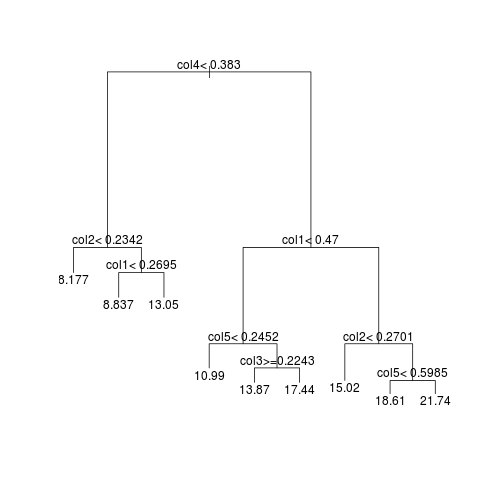
\includegraphics[totalheight=6cm]{./figs/tree_function.png}&
% 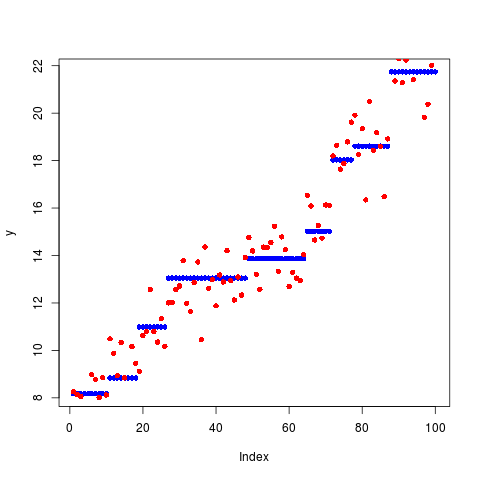
\includegraphics[totalheight=6cm]{./figs/noisy_tree_function.png}
% \end{tabular}
% \captionof{figure}{{\bf Synthetic data demonstrating RF's capability to cope with $p \gg n$.} {\bf a)} The tree
%   function, where each split means XXXX. {\bf b)} A plot of the ordered $y$ variable for the tree example, and the $y$
%   variable with added Gaussian noise (in red).}
%  \label{figure:synth}
%\end{figure}
% <<CONDENSE
%%%%%%%%%%%%%%%%%%%%%%%%%%%%%%%%%%%%%%%%%%%%%%%%%%%%%%%%%%%



%%%%%%%%%%%%%%%%%%%%%%%%%%%%%%%%
% Feature selection application example 
%%%%%%%%%%%%%%%%%%%%%%%%%%%%%%%%
%\subsection{Feature selection application example}
%Maybe we should have a feature selection on real data section. We could be using one of the smaller datasets used in the other papers?



%%%%%%%%%%%%%%%%%%%%%%%%%%%%%%%%
% Section 2: Classification selection
%%%%%%%%%%%%%%%%%%%%%%%%%%%%%%%%
\subsection{CursedForest outperforms existing methods for classification problems}
In this section we compare \cursedforest 's performance against other published methods for predicting ethnicity on the 1000 genomes dataset.


\begin{table}[!ht]
\begin{minipage}{\textwidth}
\begin{adjustwidth}{-1.25in}{0in} % Comment out/remove adjustwidth environment if table fits in text column.
\caption{
{\bf Performance comparison between the different machine learning algorithms.}}
\begin{tabular}{|p{1.2cm}|p{1cm}|p{1.5cm}+l|l|p{1.8cm}|p{1.5cm}|}
\hline
%\multicolumn{4}{|l|}{\bf Heading1} & \multicolumn{4}{|l|}{\bf Heading2}\\ \hline
\bf{Data- set} & \bf{Samp- les} & \bf{Feat- ures}  & \bf{Method} & \bf{Error (ARI)} & \bf{Runtime} & \bf{Memory/ Node} \\
\hline
%\multirow{3}{*}{phase1\_chr22: 1,092 x 490,036} & CursedForest & 0.077 (XX)  &  &  \\
phase1 chr22 &1,092 & 490,036 & CursedForest & 0.077 (XX)  & 9min 16sec & 1GB\footnote{\label{note10}10 nodes} \\
&&& RF - Spark ML & 0.069 (0.89) & 14min 13sec & 1GB\footref{note10}  \\
&&& RF - R &  0.05  & 24min  & 18GB\footref{note1}\footnote{using the \texttt{parallel} packages}\\
&&& ranger -R &         0.05 &        1min 10sec  &          16GB  (one processor) \\
 \hline
phase3 chr22 & 2,504 & 1,103,548 &  &  &  &  \\
&&& CursedForest & 0.053 & 9 min 8 sec & 2GB\footnote{\label{note20}20 nodes}\\
&&& RF - Spark ML & 0.058 (0.92) & 1hr 1min & 2GB\footref{note20} \\
&&& RF - R & NA  & NA & NA\footnote{long vectors ($> 2^31-1$)  are not supported in the .Fortran interface}\\
&&&  H2O   &        0.05 &     16 hours       &   600GB \footnote{java -Xmx600g -jar h2o.jar,   h2o.init(nthreads=20)} \\
\hline
phase3 chr1 & 2,504 & 6,450,364 & CursedForest & 0.063 (XX) & 1hr 58min & 4GB \\
&&& RF - Spark ML & (0.94) & 8hr 29min & 8GB \\
&&& LR - Spark ML&  & 2hr 6min & 8GB\\ 
&&& ranger  R   &  0.06   &     28 mins  &            num.threads = 10\footnote{don't know how to get the memory used, This
  was done on dpas-03} \\ 
\hline
phase3 chr1-3 & 2,504 & 19,328,051  & CursedForest & 0.046 (XX) & 4hr 0min & 4GB\\
&&& RF - Spark ML & - & -  & -\\
&&& LR - Spark ML & & 14hr 48min & 8GB \\ 
&&& ranger  R   &  0.05   &     58 mins\footnote{ but took 6 hours to load the data}  &      909GB\footnote{I think this is total memory. The job was run with
  ntasks-per-node=160 cores-per-socket=10 on ruby }  \\ 
\hline
phase3 chr1-22 & 2,504 & 81,047,467 & CursedForest & XX (0.96) & 7hr 14min & 8GB \\ 
&&& RF - Spark ML & - & - & - \\
&&& LR - Spark ML & - & - & - \\ 
%&&& kmeans - Spark ML & - (0.82) & 30hr 44min & 24GB \\ 
\hline
\end{tabular}
\begin{flushleft} 
Comparison of different various machine learning libraries on different subsets of variant data 
from the 1000 Genomes Project.
Each random forest model consists of 50 trees.
\end{flushleft}
\label{table1}
\end{adjustwidth}
\end{minipage}
\end{table}



%%%%%%%%%%%%%%%%%%%%%%%%%%%%%%%%
% Section 3: Sensitivity 
%%%%%%%%%%%%%%%%%%%%%%%%%%%%%%%%
\subsection{Sensitivity of parameter choice}

\begin{table}[!ht]
%\begin{adjustwidth}{-2.25in}{0in} % Comment out/remove adjustwidth environment if table fits in text column.
\caption{
{\bf Sensitivity analysis on parameter choice.}}
\begin{tabular}{|l|l|l|l|l|l|l|l|}
\hline
%\multicolumn{4}{|l|}{\bf Heading1} & \multicolumn{4}{|l|}{\bf Heading2}\\ \hline
\bf{Mtry}  & \bf{Mtree} & \bf{depth} & \bf{Accuracy} & \bf{Runtime} & \bf{Memory} \\
\hline
&&&&&\\ \hline
\end{tabular}
\begin{flushleft} 
  Table notes here.
\end{flushleft}
\label{table2}
%\end{adjustwidth}
\end{table}




\section{Conclusion}




\section{Supporting Information}

% Include only the SI item label in the subsection heading. Use the \nameref{label} command to cite SI items in the text.
%\subsection*{S1 Video}
%\label{S1_Video}
%{\bf Bold the first sentence.}  Maecenas convallis mauris sit amet sem ultrices gravida. Etiam eget sapien nibh. Sed ac ipsum eget %enim egestas ullamcorper nec euismod ligula. Curabitur fringilla pulvinar lectus consectetur pellentesque.


\section*{Acknowledgments}
Cras egestas velit mauris, eu mollis turpis pellentesque sit amet. Interdum et malesuada fames ac ante ipsum primis in faucibus. Nam id pretium nisi. Sed ac quam id nisi malesuada congue. Sed interdum aliquet augue, at pellentesque quam rhoncus vitae.

\nolinenumbers

\bibliography{./CursedForest.bib}

\end{document}





%  \item D\iaz-Uriarte, R., \& Alvarez de Andr\es, S. (2006). Gene selection and classification of microarray data using random
%    forest. BMC Bioinformatics, 7, 3. http://doi.org/10.1186/1471-2105-7-3
%  \item Goldstein, B. A., Polley, E. C., & Briggs, F. B. S. (2011). Random Forests for Genetic Association Studies. Statistical
%    Applications in Genetics and Molecular Biology, 10(1), 32. http://doi.org/10.2202/1544-6115.1691



%@article{Chen2012323,
%title = "Random forests for genomic data analysis ",
%journal = "Genomics ",
%volume = "99",
%number = "6",
%pages = "323 - 329",
%year = "2012",
%note = "",
%issn = "0888-7543",
%doi = "http://dx.doi.org/10.1016/j.ygeno.2012.04.003",
%url = "http://www.sciencedirect.com/science/article/pii/S0888754312000626",
%author = "Xi Chen and Hemant Ishwaran",
%keywords = "Random forests",
%keywords = "Random survival forests",
%keywords = "Classification",
%keywords = "Prediction",
%keywords = "Variable selection",
%keywords = "Genomic data analysis ",
%abstract = "Random forests (RF) is a popular tree-based ensemble machine learning tool that is highly data adaptive, applies to “large p, small n” problems, and is able to account for correlation as well as interactions among features. This makes \{RF\} particularly appealing for high-dimensional genomic data analysis. In this article, we systematically review the applications and recent progresses of \{RF\} for genomic data, including prediction and classification, variable selection, pathway analysis, genetic association and epistasis detection, and unsupervised learning. "
%}


%http://stats.stackexchange.com/questions/77018/random-forest-is-it-a-boosting-algorithm
 %http://stats.stackexchange.com/questions/173390/gradient-boosting-tree-vs-random-forest
%overcomes this issue and is hence ideally suited to this application.  Furthermore, RF are able to capture interactions
%between features, which is of importance for modelling complex polygenic diseases.


% We also investigated classifying the samples using Random Forests.  We chose random forests due to its ability to
% capture complex interactions between features. Also, due to it being an ensemble method where trees can be formed
% independently, which, is ideal for parallelisation. Furthermore, the ensemble of weak learners can help to minimise
% overfitting and variance.



% The reason for the failure can be attributed to the "curse of dimensionality". Where Spark ML is designed to process a
% huge number of samples with a modest dimensionality, the 1000 Genomes data instead contains a huge number of
% dimensions (features). As a result, the default random forests implementation is unable to partition the data into
% small-enough tasks for nodes on the computer cluster to handle.



% For figure citations, please use "Fig." instead of "Figure".
%Nulla mi mi, Fig.~\ref{fig1}  Fusce fringilla erat porttitor lectus cursus, \nameref{S1_Video} vel sagittis arcu lobortis. Aliquam in enim semper, aliquam massa id, cursus neque. Praesent faucibus semper libero.
%\begin{figure}[h]
%\caption{{\bf Figure Title first bold sentence Nulla mi mi, venenatis sed ipsum varius, volutpat euismod diam.}
%Figure Caption Proin rutrum vel massa non gravida. Quisque tempor sem et dignissim rutrum. A: Lorem ipsum dolor sit amet. B: Consectetur adipiscing elit.}
%\label{fig1}
%\end{figure}
%\begin{enumerate}
%\item{react}
%\item{diffuse free particles}
%\item{increment time by dt and go to 1}
%\end{enumerate}

% Results and Discussion can be combined.
% Please do not create a heading level below \subsection. For 3rd level headings, use \paragraph{}. 



%\begin{table}[!ht]
%\begin{adjustwidth}{-2.25in}{0in} % Comment out/remove adjustwidth environment if table fits in text column.
%\caption{
%{\bf Table caption Nulla mi mi, venenatis sed ipsum varius, volutpat euismod diam.}}
%\begin{tabular}{|l|l|l|l|l|l|l|l|}
%\hline
%\multicolumn{4}{|l|}{\bf Heading1} & \multicolumn{4}{|l|}{\bf Heading2}\\ \hline
%$cell1 row1$ & cell2 row 1 & cell3 row 1 & cell4 row 1 & cell5 row 1 & cell6 row 1 & cell7 row 1 & cell8 row 1\\ \hline
%$cell1 row2$ & cell2 row 2 & cell3 row 2 & cell4 row 2 & cell5 row 2 & cell6 row 2 & cell7 row 2 & cell8 row 2\\ \hline
%$cell1 row3$ & cell2 row 3 & cell3 row 3 & cell4 row 3 & cell5 row 3 & cell6 row 3 & cell7 row 3 & cell8 row 3\\ \hline
%\end{tabular}
%\begin{flushleft} Table notes Phasellus venenatis, tortor nec vestibulum mattis, massa tortor interdum felis, nec pellentesque metus tortor nec nisl. Ut ornare mauris tellus, vel dapibus arcu suscipit sed.
%\end{flushleft}
%\label{table1}
%\end{adjustwidth}
%\end{table}
